% Définition du répertoire contenant les images
\graphicspath{{IMAGE/}}

% FRAME Intro
\begin{frame}


\includegraphics[width=12cm]{Logos.pdf}

\vfill

\begin{center}

\vspace*{1.5cm}

\LARGE
\textbf{Density}

\vspace*{1.5cm}
 DELHI GIS-R School


\large
9-12\up{th} April 2019

\vspace*{1.5cm}


\textbf{Hadrien Commenges \& Paul Chapron}

{\small

\vspace*{0.1cm}

\url{hadrien.commenges@univ-paris1.fr}

\url{paul.chapron@ign.fr}
}

\end{center}

\end{frame}

% FRAME
\begin{frame}{Use case}

\begin{block}{Density}
Density is a \textbf{spatial variable} depicting the \textbf{spatial variation} of some observations (concentration and dispersion) in 1, 2 or $n$ dimensions. 
\end{block}

\begin{itemize}
\item Mass / Volume ratio (volumetric mass), mass per volume unit, sometimes ratio between an object volumetric mass and a reference volumetric mass. 
\item Ratio between a \textbf{count}  and its \textbf{extent}: a variable's density (1D), population density (2D, so \textbf{spatial extent}), etc.
\end{itemize}

~

\textbf{What kind of geographical information is concerned ?}

$\rightarrow$ \textit{TYPE 1 - Geographical Objects}

$\rightarrow$ \textit{TYPE 2 - Occurrences}

\end{frame}


% FRAME
\begin{frame}{Goals}

\textbf{Main uses:}

\begin{enumerate}
  \item Describe a point pattern 
  \item Estimate the probability of an event to occur at a given point
  \item Estimate the probability that a spatial distribution of events is random.
\end{enumerate}

\end{frame}


% FRAME
\begin{frame}{Spatial distribution parameters}

\textbf{Centrality} and \textbf{dispersion} can be computed in a 1, 2 2 or $n$ dimensions space. 

~

Current analysis of these parameters:

\begin{itemize}
\item Description of a distribution: mean and standard deviation
\item Evolution of these parameters over time
\item Parameters weight
\end{itemize}

\end{frame}


% FRAME
\begin{frame}{Paramètres d'une distribution}

Calcul de la \textbf{moyenne} en deux dimensions : \textbf{point moyen} ou \textbf{barycentre}.

$$
x_g = \frac{\sum_{i=1}^n w_i x_i}{\sum_{i=1}^n w_i} ~~~~~~~~~~~~~~~ y_g = \frac{\sum_{i=1}^n w_i y_i}{\sum_{i=1}^n w_i}
$$

~

~

$\rightarrow$ Les poids $w_i$ peuvent être constants ou variables, exprimant la variation d'un stock localisé.

\end{frame}



% FRAME
\begin{frame}{Paramètres d'une distribution}

Calcul de la \textbf{variance} en deux dimensions : \textbf{inertie}.

\begin{figure}
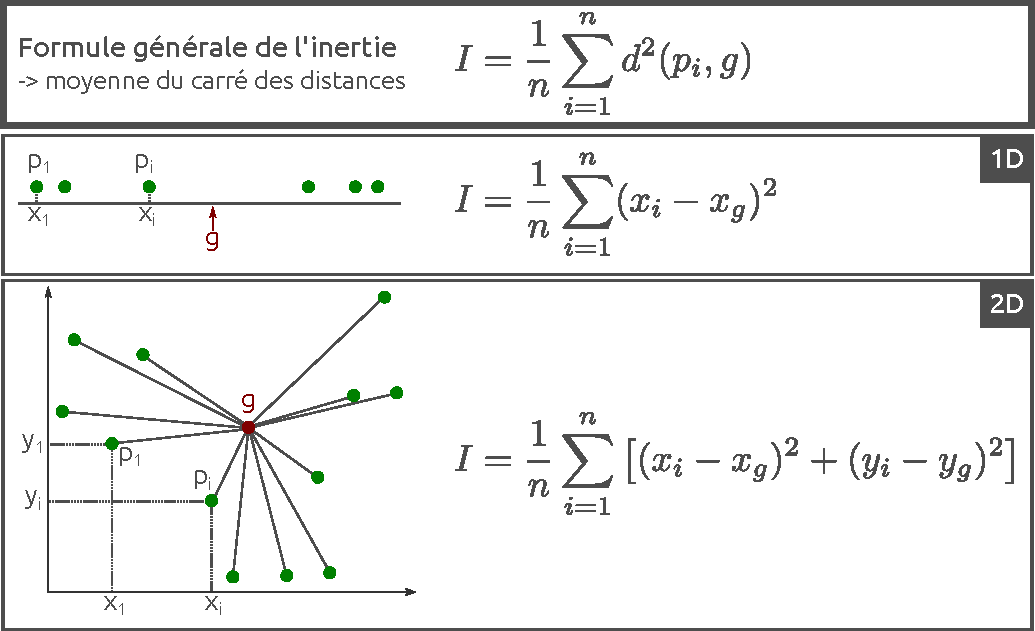
\includegraphics[width=11cm]{Inertie.pdf}
\end{figure}


\end{frame}

% FRAME
\begin{frame}{Paramètres d'une distribution}

\begin{figure}
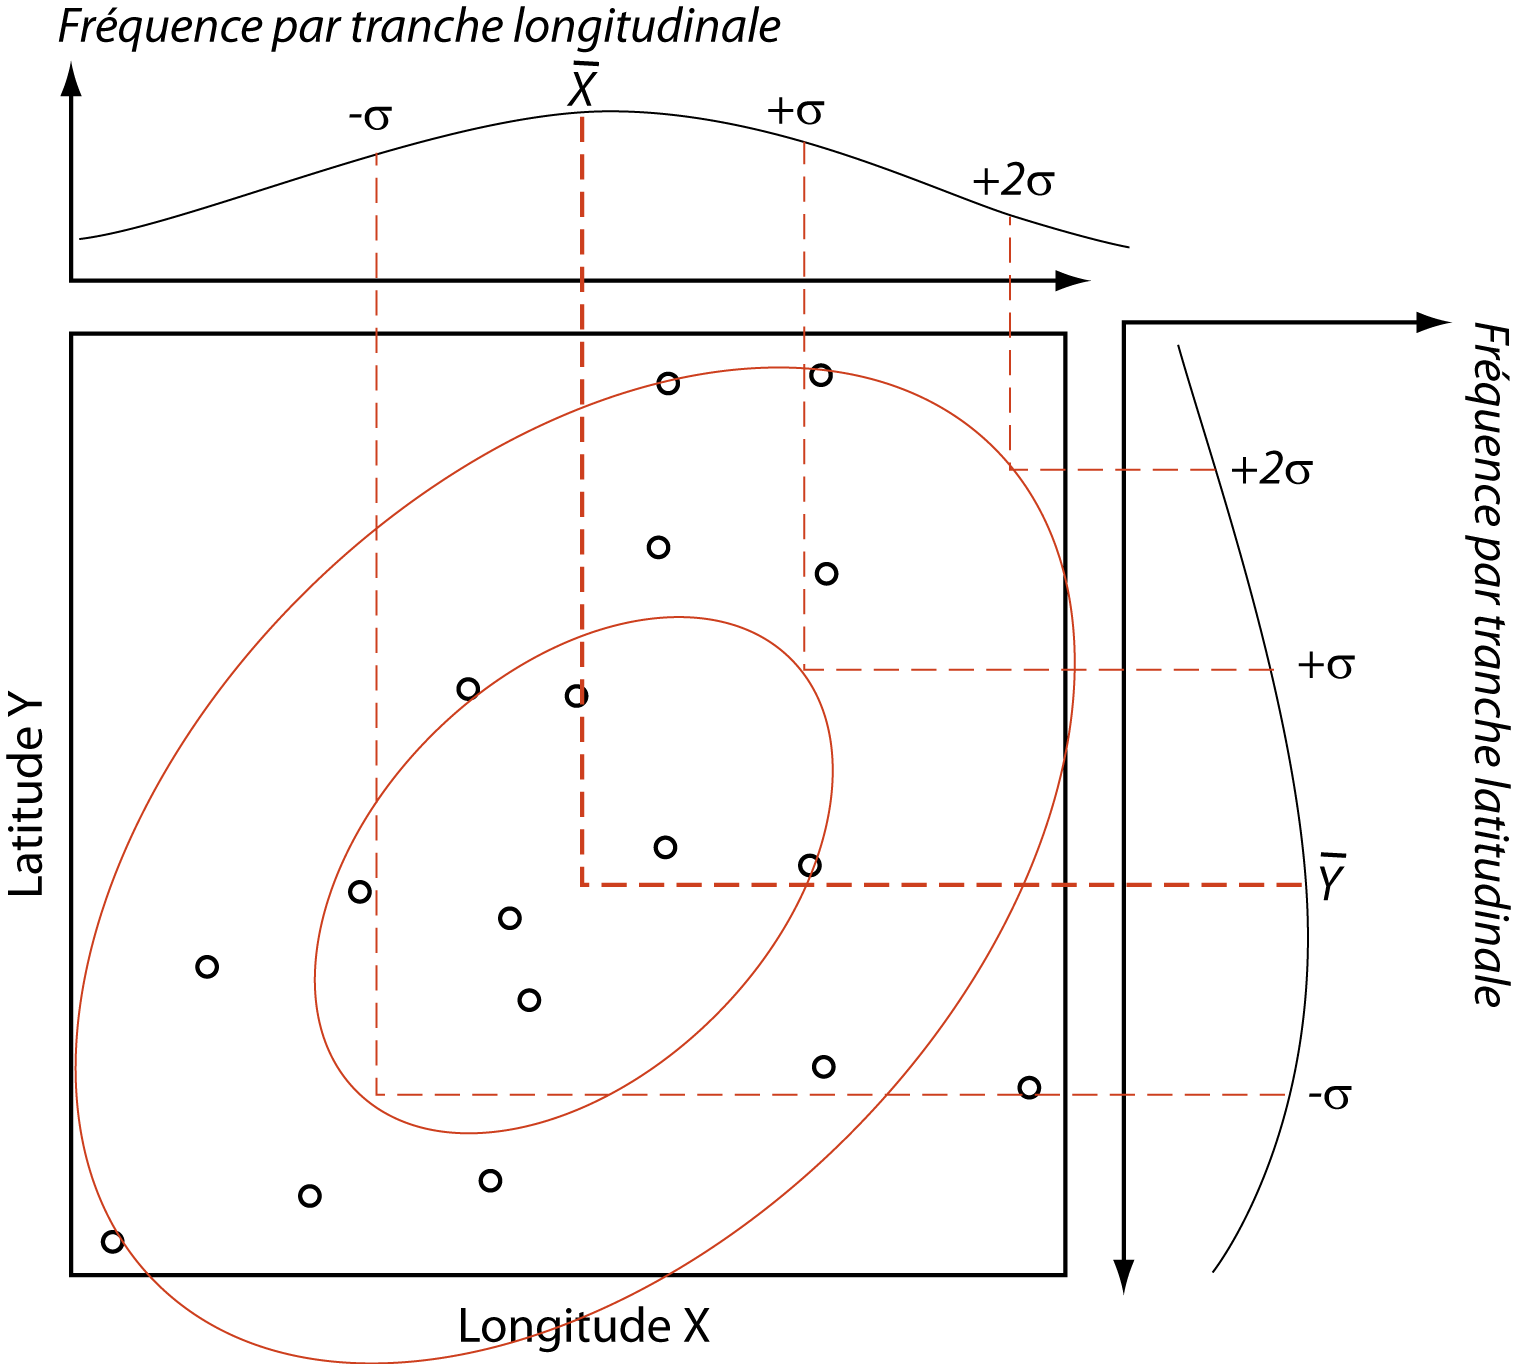
\includegraphics[width=9cm]{EllipseStandard.png}
\end{figure}

\end{frame}


% FRAME
\begin{frame}{Paramètres d'une distribution}

\begin{figure}
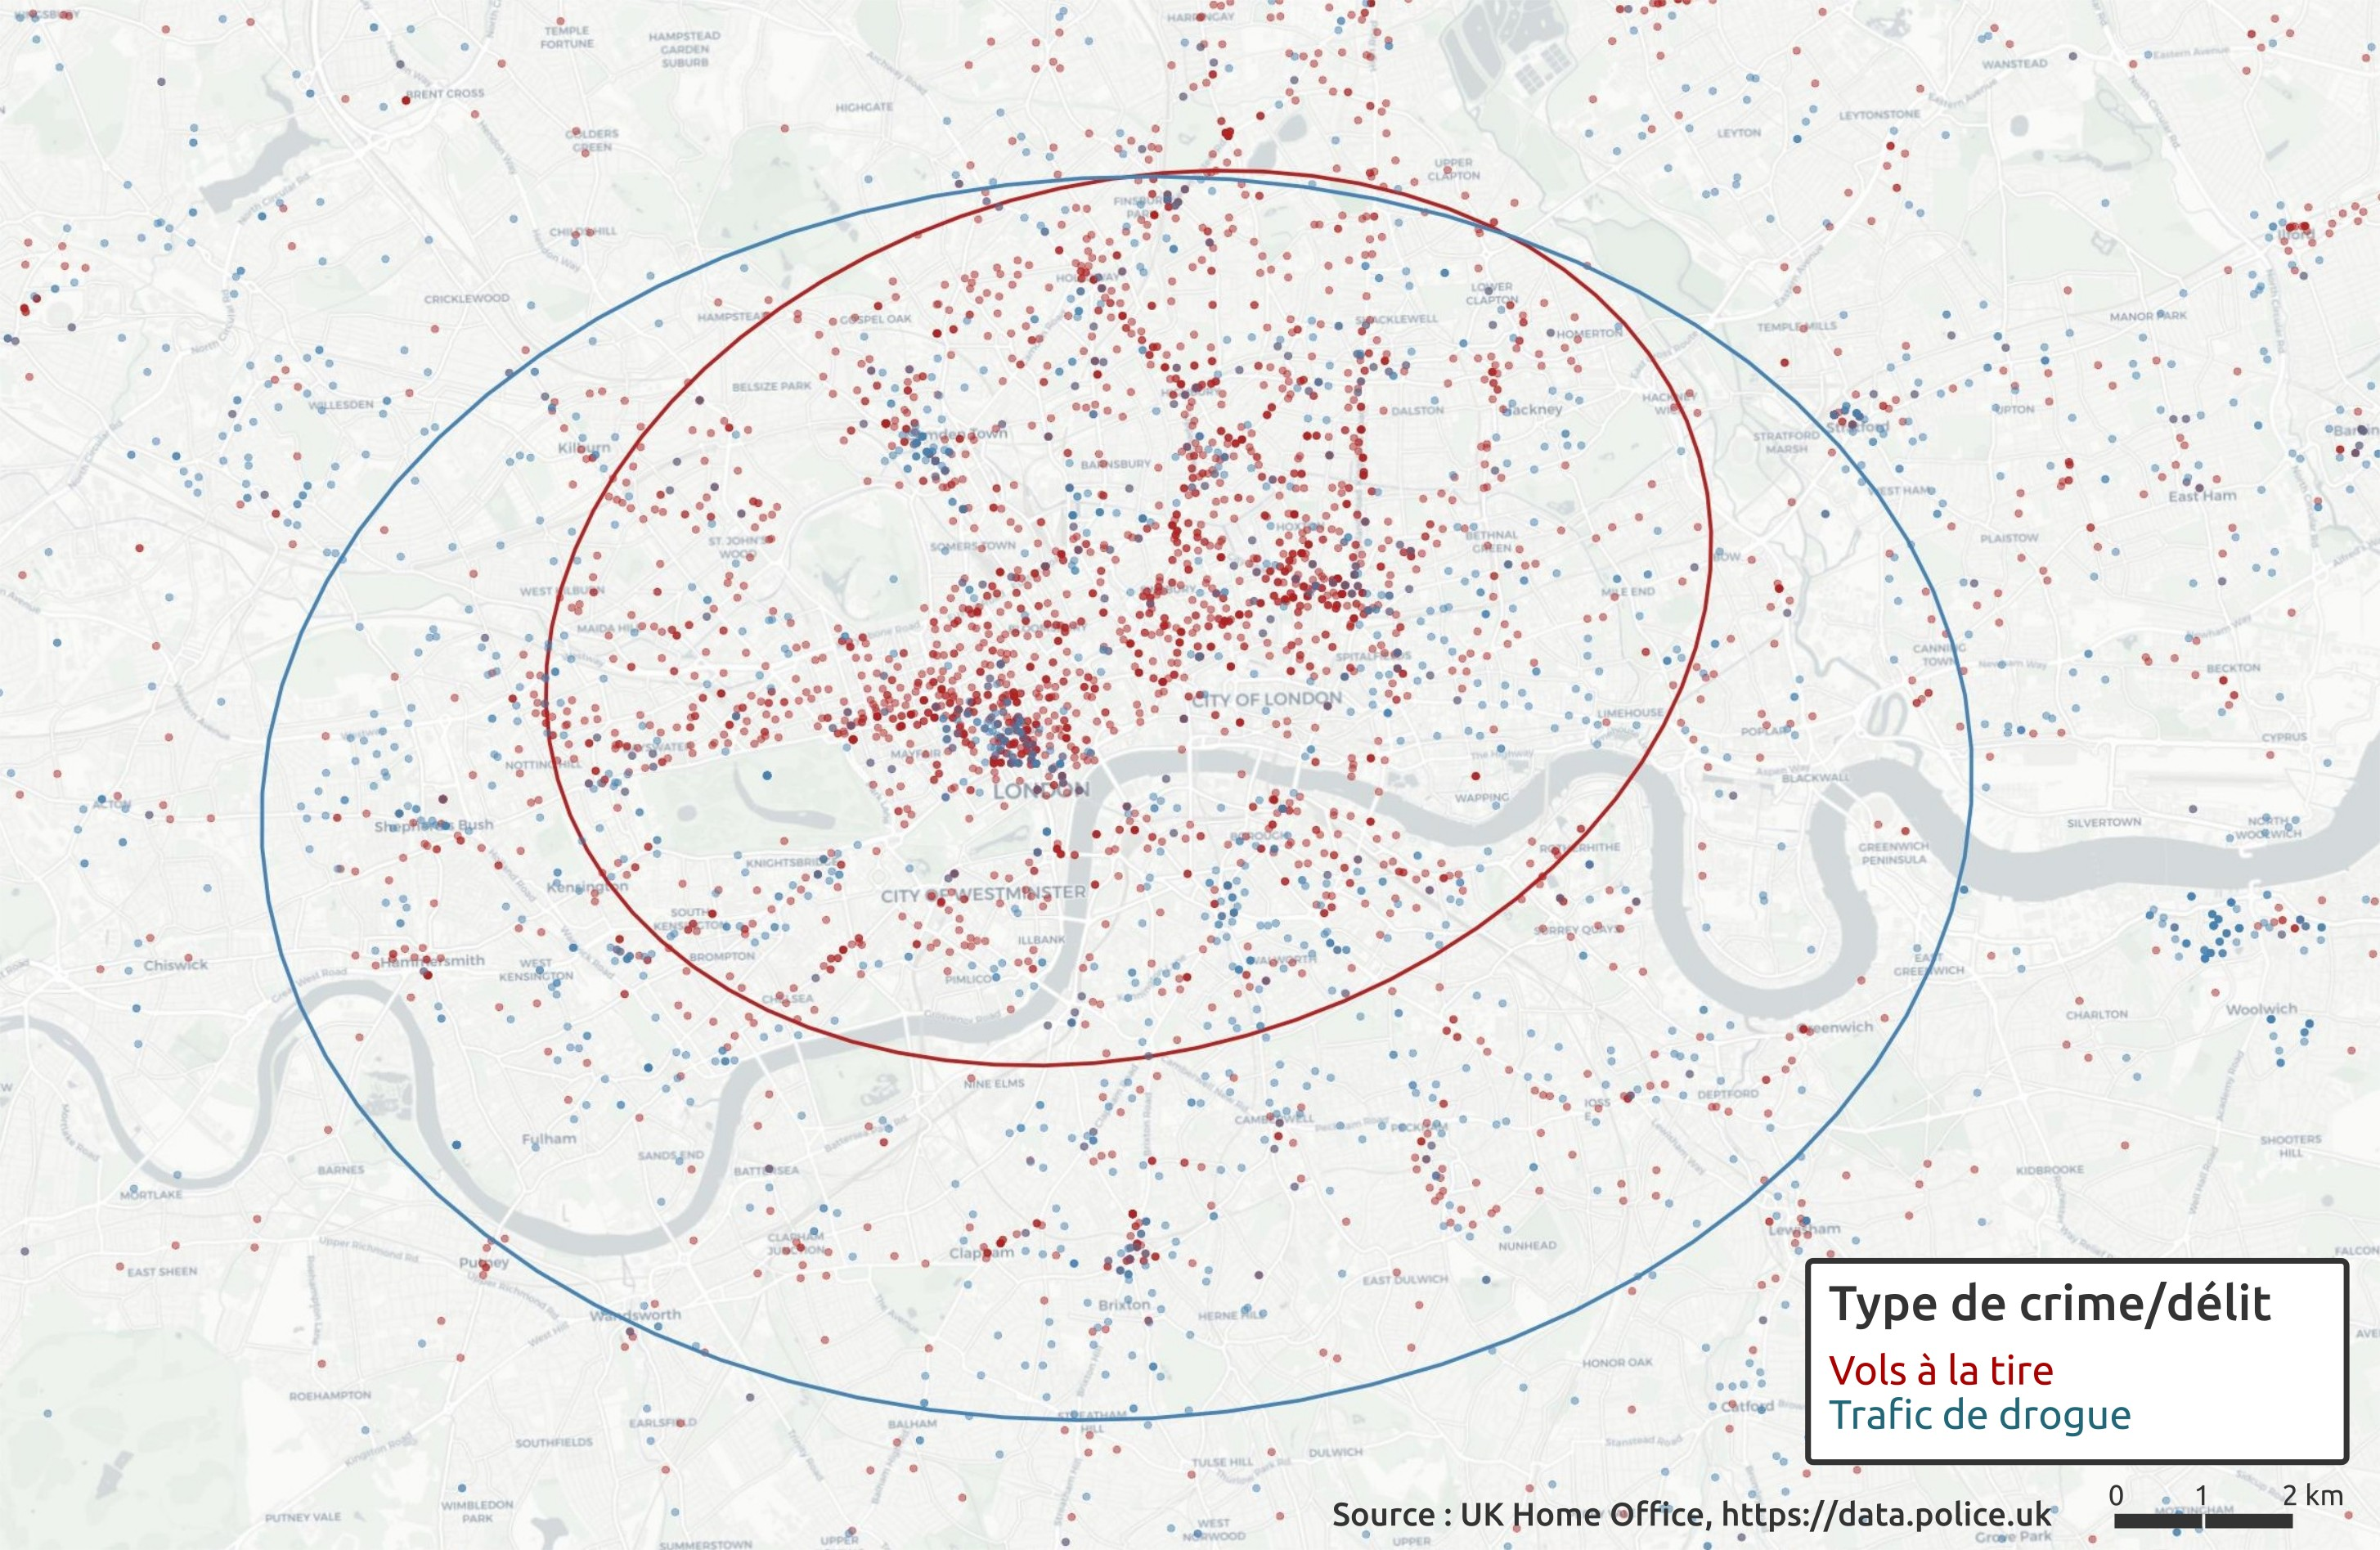
\includegraphics[width=12cm]{Crimes.jpg}
\end{figure}

\end{frame}



% FRAME
\begin{frame}{Paramètres d'une distribution}

\begin{figure}
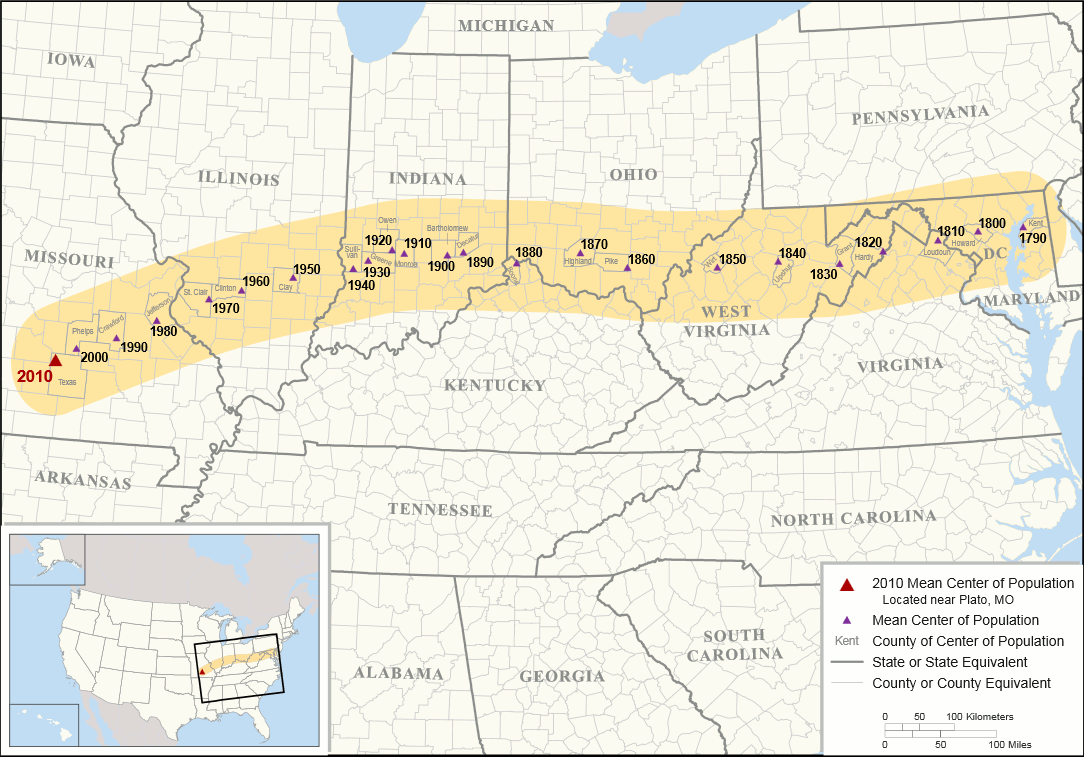
\includegraphics[width=10cm]{Centerpop.png}
\end{figure}

\footnotesize
Source: US Census, \url{https://www.census.gov/geo/reference/centersofpop.html}
\normalsize

\end{frame}


% FRAME
\begin{frame}{Graphier une distribution (discret)}

\textbf{Qu'est-ce qu'un histogramme?}

~ 

\begin{figure}
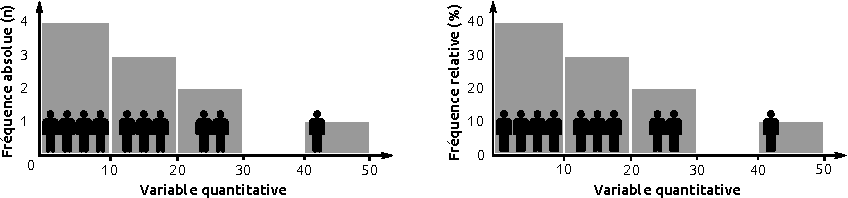
\includegraphics[width=12cm]{Histogramme.pdf}
\end{figure}

$\rightarrow$ La densité estimée par l'histogramme est par construction \textbf{discontinue}.

\end{frame}


% FRAME
\begin{frame}{Graphier une distribution (Parzen)}

\textbf{Généralisation de l'histogramme: fenêtre de Parzen}

~ 

\begin{figure}
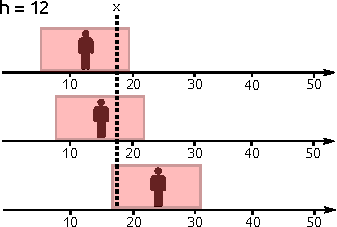
\includegraphics[width=6cm]{HistogrammeParzen.pdf}
\end{figure}

~

$$ D(x) = \frac{1}{3 \times 12} (1 + 1 + 1) = \frac{1}{12}$$

\end{frame}



% FRAME
\begin{frame}{Graphier une distribution (Parzen)}

\textbf{Généralisation de l'histogramme: fenêtre de Parzen}

~ 

\begin{figure}
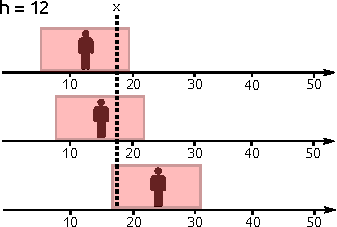
\includegraphics[width=6cm]{HistogrammeParzen.pdf}
\end{figure}

$$ D(x) = \frac{1}{3 \times 12} (1 + 1 + 1) = \frac{1}{12}$$

\end{frame}


% FRAME
\begin{frame}{Graphier une distribution (continu)}

\textbf{Généralisation de Parzen: noyau gaussien}

\begin{figure}
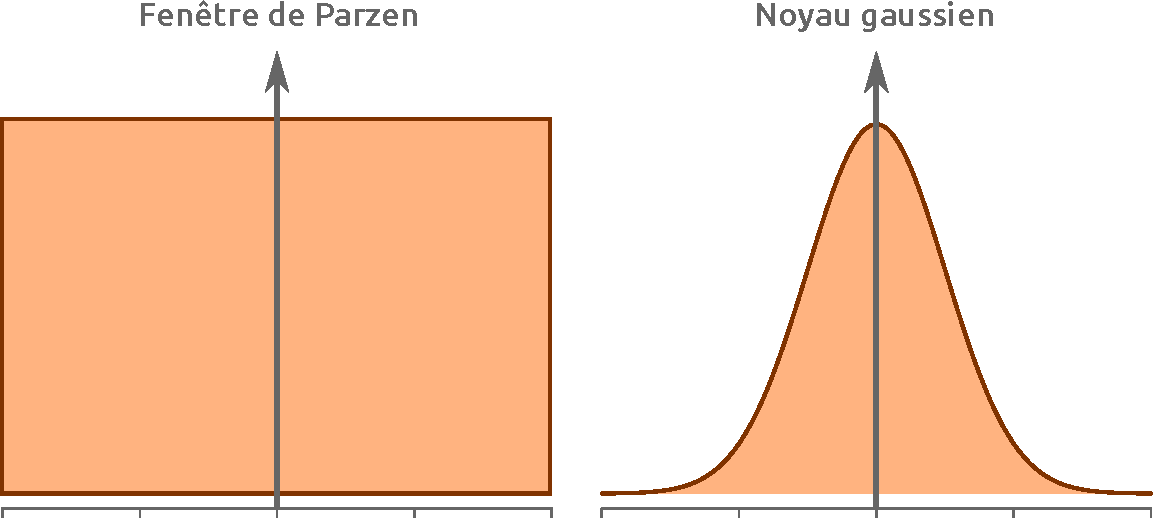
\includegraphics[width=10cm]{Gauss.pdf}
\end{figure}

\end{frame}


% FRAME
\begin{frame}{Graphier une distribution (continu)}

\textbf{Généralisation de Parzen: noyau gaussien}

\begin{figure}
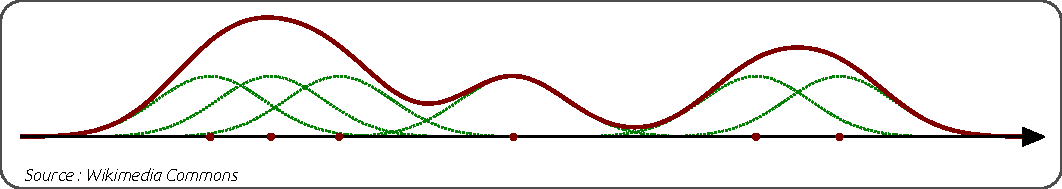
\includegraphics[width=12cm]{KDE.pdf}
\end{figure}

~

L'estimation du noyau (KDE - \textit{Kernel Density Estimator}) est applicable en 1 ou en n dimensions. En analyse spatiale on l'utilisera en \textbf{2 dimensions}.

\end{frame}


% FRAME
\begin{frame}{Cartographier une distribution}

Densité par estimateur du noyau (KDE) en \textbf{deux dimensions}.

\begin{figure}
  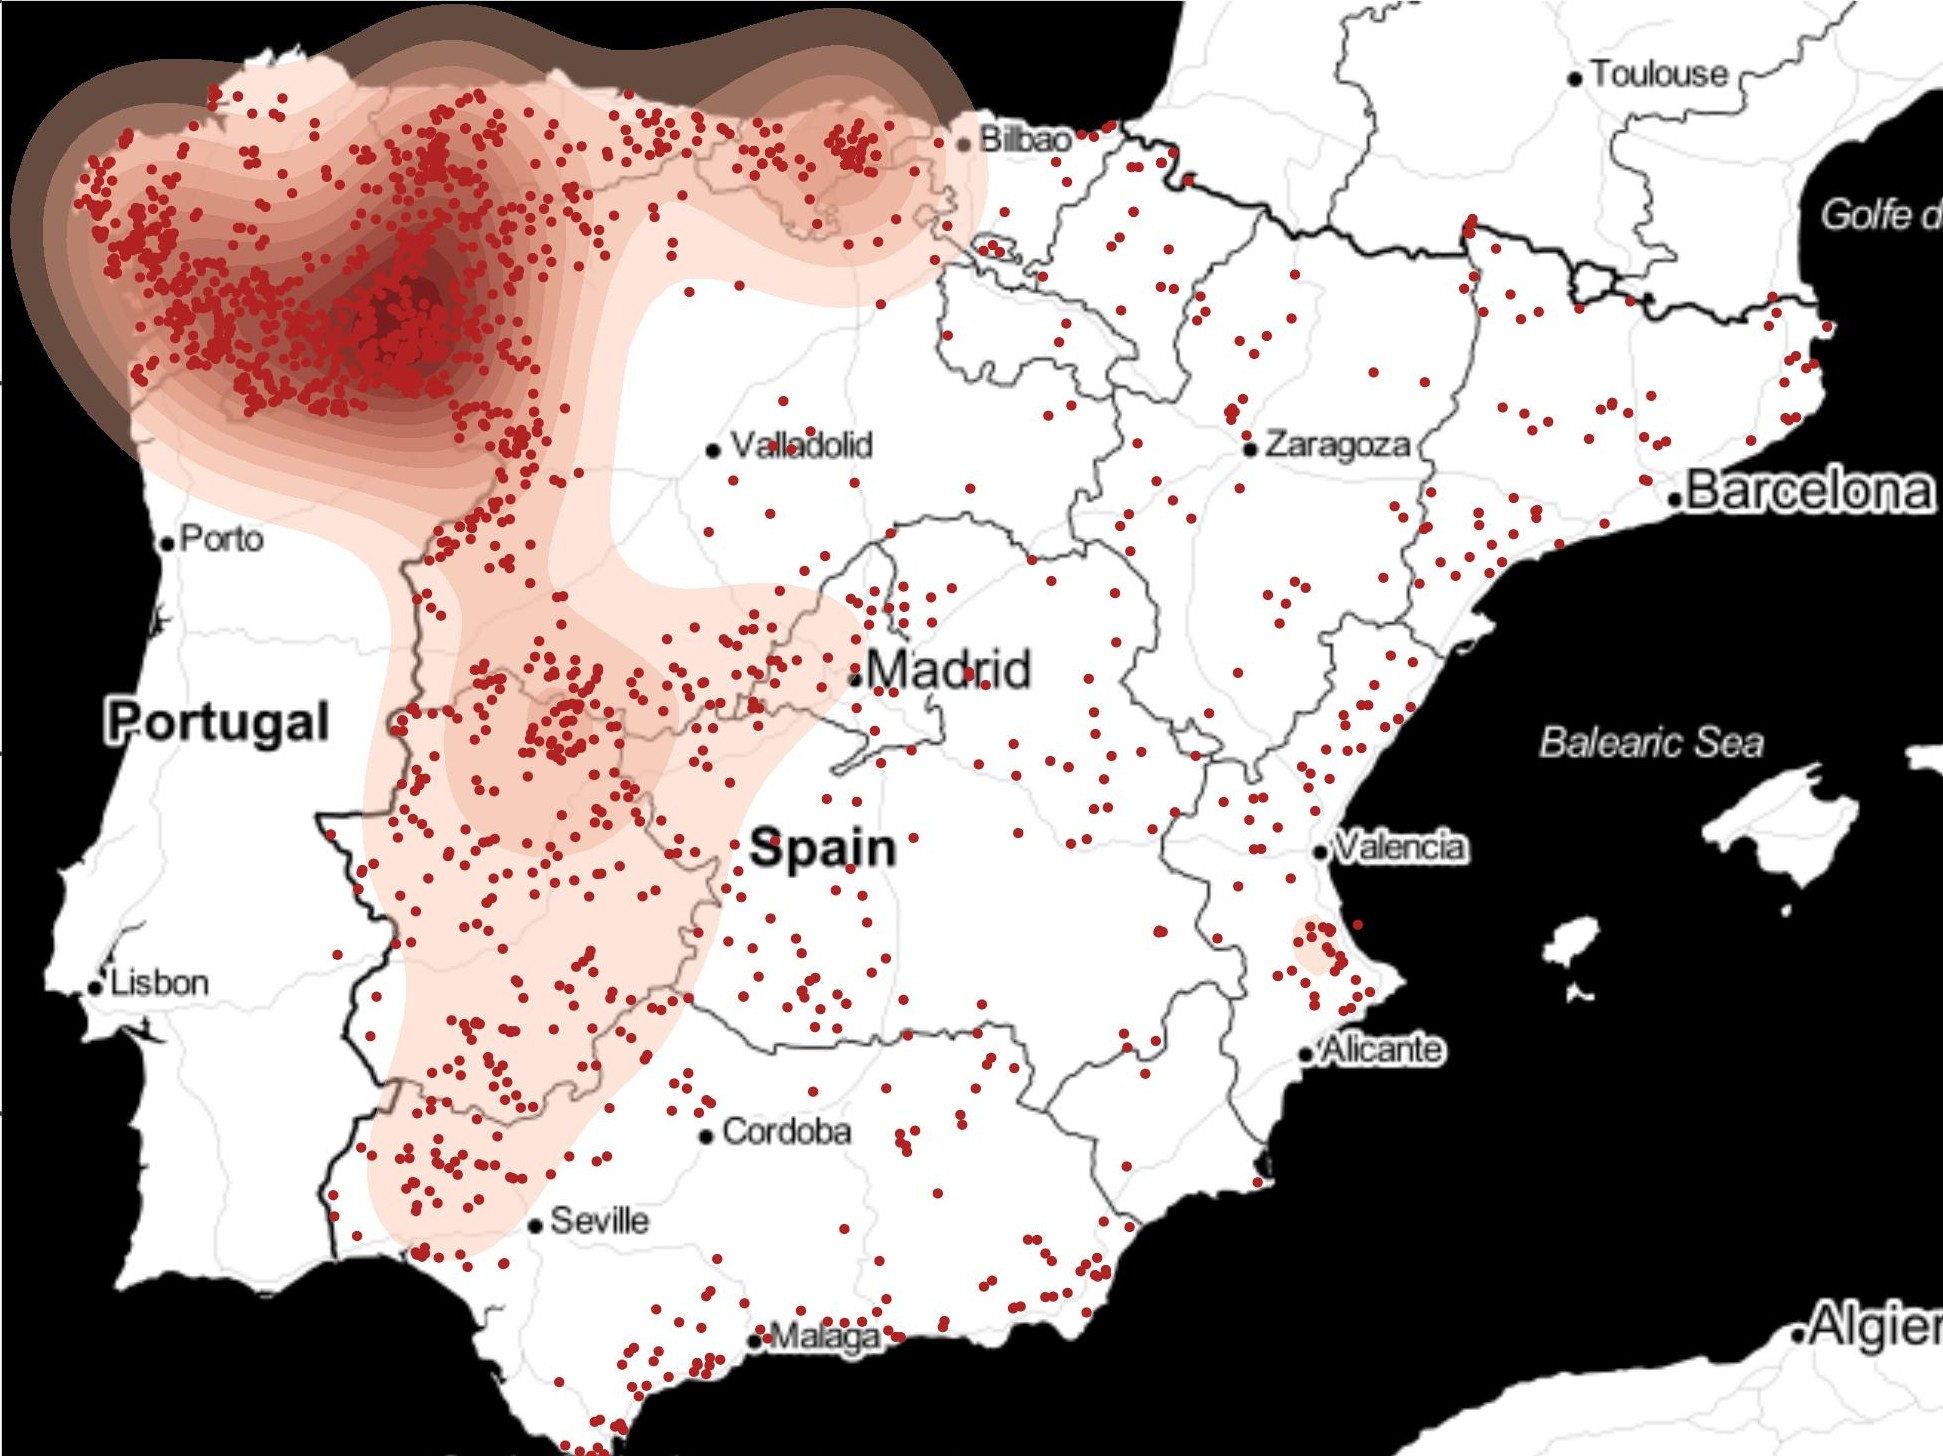
\includegraphics[width=8cm]{Incendies.jpg}
\end{figure}

\end{frame}


% FRAME
\begin{frame}{Tester une distribution}

\textbf{La distribution peut-elle être produite par un processus aléatoire?}

\begin{figure}
  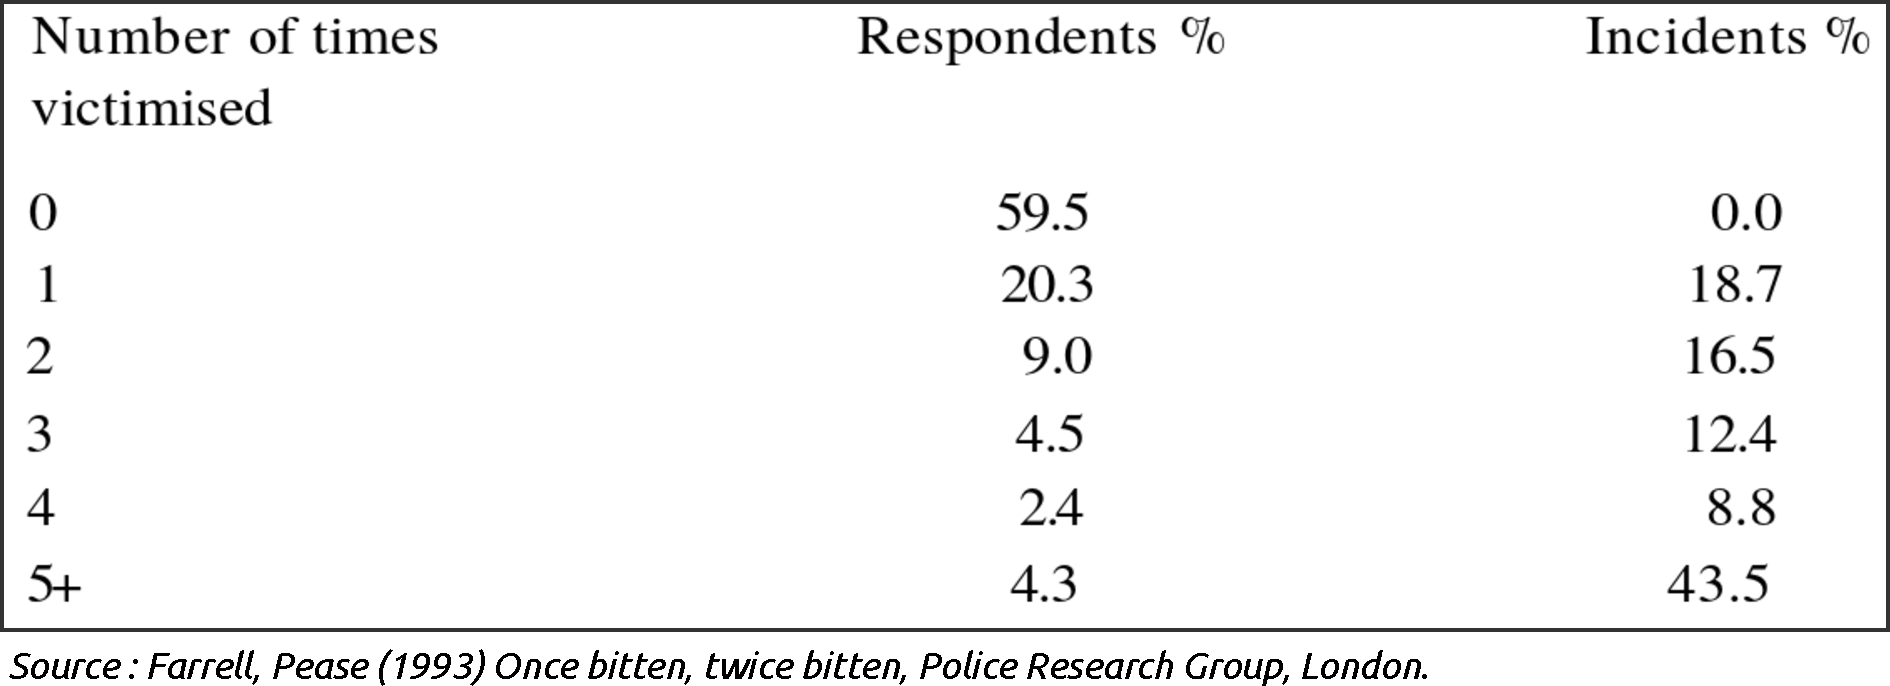
\includegraphics[width=11cm]{CrimeConcentration.pdf}
\end{figure}

\end{frame}


% FRAME
\begin{frame}{Tester une distribution}

\textbf{La distribution peut-elle être produite par un processus aléatoire?}

\begin{figure}
  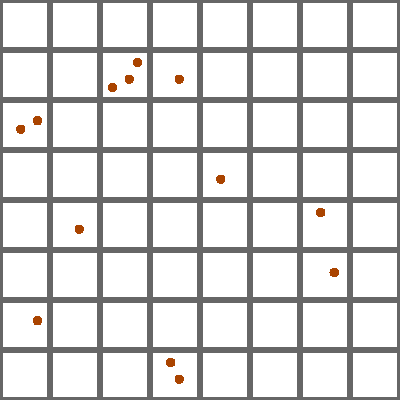
\includegraphics[width=6.5cm]{ExPoisson.pdf}
\end{figure}

\end{frame}


% FRAME
\begin{frame}{Tester une distribution}

\textbf{La distribution peut-elle être produite par un processus aléatoire?}

\begin{figure}
  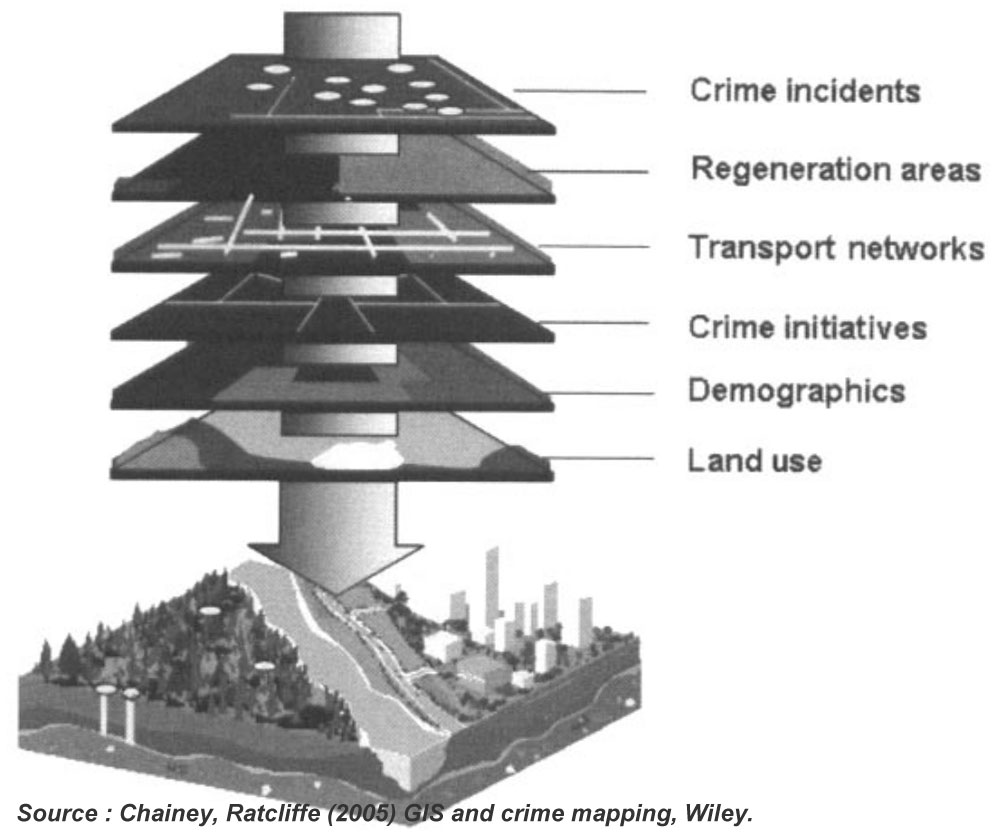
\includegraphics[width=7cm]{Chainey.jpg}
\end{figure}

\end{frame}


% FRAME
\begin{frame}{Distribution statistique de Poisson}

La distribution de Poisson se définit par un seul paramètre $\lambda$ qui est à la fois la moyenne et la variance de la distribution.

\begin{equation}
\nonumber
P(X = k) = \frac{\lambda^k e^{-\lambda}}{k!}
\end{equation}


\begin{figure}
  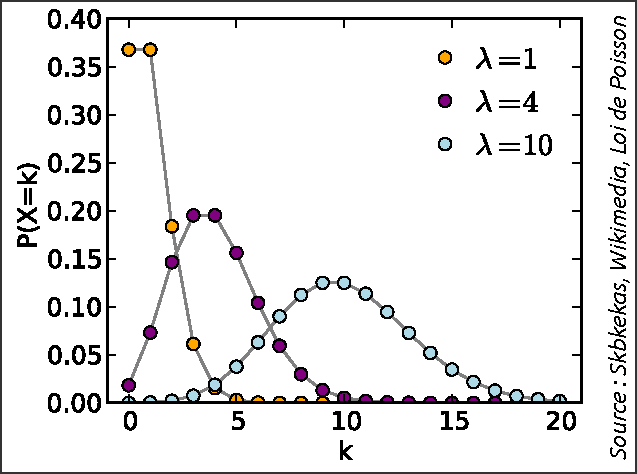
\includegraphics[width=7cm]{Poisson.pdf}
\end{figure}

\end{frame}



% FRAME
\begin{frame}{Distribution spatiale de Poisson}

Un \textbf{processus de spatial de Poisson} est un processus \textbf{spatialement aléatoire}, en anglais on trouve les termes suivants:

\begin{itemize}
  \item \textit{spatial Poisson process}
  \item \textit{homogeneous Poisson process}
  \item \textit{complete spatial randomness} (CSR)
\end{itemize}

Dans un espace découpé en zones, on estime la probabilité d'un nombre d'occurrences (points) dans une zone par une distribution de poisson de moyenne $\lambda \times surface(zone)$.

\end{frame}


% FRAME
\begin{frame}{Indicateur de dispersion}

\textbf{Calcul de l'indicateur VMR} \textit{Variance-to-Mean Ratio}

\begin{itemize}
\item Carroyer l'espace d'étude
\item Dénombrer les occurrences
\item Calculer la variance, la moyenne et le ratio variance/moyenne
\end{itemize}

~

\textbf{Interprétation du VMR}

\begin{itemize}
  \item VMR = 1 \\ distribution possiblement produite par un processus de Poisson
  \item VMR < 1 \\ distribution à tendance homogène
  \item VMR > 1 \\ distribution à tendance concentrée
\end{itemize}

\end{frame}


% FRAME
\begin{frame}{Indicateur de dispersion}

\begin{figure}
  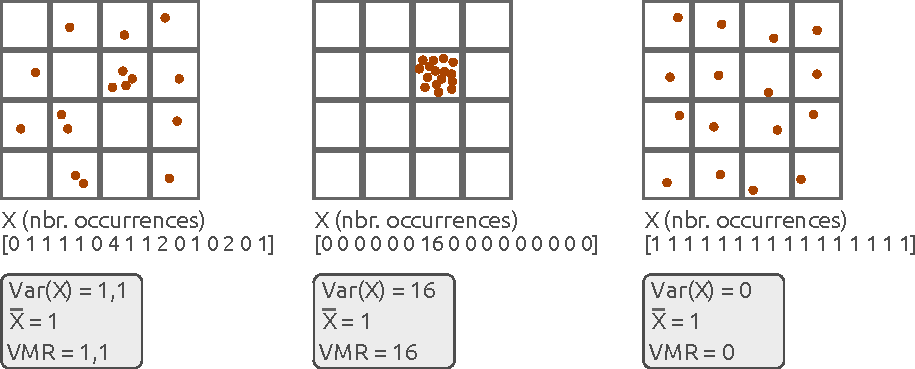
\includegraphics[width=12cm]{VMR.pdf}
\end{figure}

$\rightarrow$ \textbf{test:} le VMR est-il significativement différent de 1? (test de Student)

\end{frame}


% FRAME
\begin{frame}{Méthode des quadrats}

\textbf{Calcul des quadrats}

\begin{itemize}
  \item Carroyer l'espace d'étude (quadrats).
  \item Le modèle de référence, modèle nul, qui donne les valeurs espérées dans la grille, est le processus spatial de Poisson.
  \item On obtient tableaux de contingence avec un compte d'occurrences (observé, espéré).
\end{itemize}

$\rightarrow$ \textbf{test:} les valeurs observées sont-elles significativement différentes des valeurs espérées (test du $\chi^2$)

\end{frame}

